\documentclass[11pt,a4paper]{article}

% Configuración de página y márgenes
\usepackage[margin=1in, top=1.2in, bottom=1.2in]{geometry}

% Paquetes para caracteres especiales y codificación
\usepackage[utf8]{inputenc}
\usepackage[T1]{fontenc}
\usepackage{lmodern}
\usepackage{textcomp}
\usepackage{amsma% Pie de página
\fancyfoot[L]{\small UNIT Electronics - Development}
\fancyfoot[C]{\small 2025-07-21}
\fancyfoot[R]{\small Page \thepage\ of \pageref{LastPage}}

% Línea en encabezado y pie
\renewcommand{\headrulewidth}{0.4pt}
\renewcommand{\footrulewidth}{0.4pt}

% Estilo para primera página de cada sección
\fancypagestyle{plain}{
    \fancyhf{}
    \fancyfoot[L]{\small UNIT Electronics - Development}
    \fancyfoot[C]{\small 2025-07-21}
    \fancyfoot[R]{\small Page \thepage\ of \pageref{LastPage}}
    \renewcommand{\headrulewidth}{0pt}
    \renewcommand{\footrulewidth}{0.4pt}
}ssymb}
\usepackage{gensymb}

% Soporte para idiomas (español e inglés)
\usepackage[spanish,english]{babel}

% Paquetes para imágenes y gráficos
\usepackage{graphicx}
\usepackage{float}
\usepackage{caption}
\usepackage{subcaption}

% Paquetes para tablas
\usepackage{longtable}
\usepackage{booktabs}
\usepackage{array}
\usepackage{multirow}
\usepackage{multicol}
\usepackage{tabularx}

% Control de saltos de página
\usepackage{needspace}
\usepackage{afterpage}
\usepackage{placeins}

% Enlaces e hipervínculos
\usepackage[colorlinks=true, linkcolor=blue, urlcolor=blue, citecolor=blue]{hyperref}

% Paquetes para código y verbatim
\usepackage{fancyvrb}
\usepackage{listings}
\usepackage{xcolor}

% Paquetes para diseño profesional
\usepackage{tcolorbox}
\usepackage{tikz}
\tcbuselibrary{most}
\usepackage{fancyhdr}
\usepackage{lastpage}

% Configuración de listings para código
\lstset{
    basicstyle=\ttfamily\small,
    breaklines=true,
    frame=single,
    backgroundcolor=\color{gray!10},
    keywordstyle=\color{blue},
    commentstyle=\color{green!50!black},
    stringstyle=\color{red}
}

% Paquetes para mejor tipografía
\usepackage{microtype}
\usepackage{setspace}

% Configuración de espaciado
\onehalfspacing

% Comandos personalizados
\providecommand{\tightlist}{}

% Comando para evitar viudas y huérfanas
\widowpenalty=10000
\clubpenalty=10000

% Configuración de profundidad de numeración
\setcounter{secnumdepth}{3}
\setcounter{tocdepth}{3}

\begin{document}


% Página de título estandarizada IEEE/ISO
\begin{titlepage}
    \centering
    
    % Header corporativo estandarizado
    \vspace*{0.5cm}
    
    % Logo y información corporativa
    \begin{minipage}{0.3\textwidth}
        \centering
        $if(logo)$
        
\includegraphics[width=\textwidth]{logo.png}
        
    \end{minipage}
    \hfill
    \begin{minipage}{0.6\textwidth}
        \raggedleft
        {\small \textbf{UNIT Electronics}}\\
        {\footnotesize Technical Documentation}\\
        {\footnotesize Development Project - Prototype Phase}
    \end{minipage}
    
    \vspace{0.5cm}
    
    % Línea divisoria principal
    {\color{blue}\rule{\textwidth}{2pt}}
    
    \vspace{1.5cm}
    
    % Clasificación del documento
    \begin{tcolorbox}[
        colback=blue!5!white,
        colframe=blue!75!black,
        width=0.9\textwidth,
        arc=2mm,
        boxrule=1.5pt,
        halign=center
    ]
    {\Large \textbf{TECHNICAL DATASHEET}}\\[0.2cm]
    {\normalsize Hardware Documentation \& Development Specifications}
    \end{tcolorbox}
    
    \vspace{0.8cm}
    
    % Título principal estandarizado
    {\Huge \textbf{\textcolor{blue}{ICP-10111 Barometric Pressure Sensor}}}\\[0.3cm]
    
    % Subtítulo técnico
    
    {\LARGE \textcolor{gray}{High-Precision Environmental Sensor Module}}\\[0.5cm]
    
    
    % Código de parte y versión
    \begin{tcolorbox}[
        colback=gray!10!white,
        colframe=gray!50!black,
        width=0.7\textwidth,
        arc=1mm,
        boxrule=1pt
    ]
    \centering
    \begin{tabular}{l l}
    \textbf{Part Number:} & ICP-10111-001 \\
    \textbf{Revision:} & Rev. 1.0 \\
    \textbf{Document Date:} & 2025-07-21
    \end{tabular}
    \end{tcolorbox}
    
    \vspace{1cm}
    
    % Tabla de información del documento (Formato simplificado)
    \begin{tcolorbox}[
        colback=white,
        colframe=black,
        width=0.9\textwidth,
        arc=0mm,
        boxrule=1pt,
        halign=center
    ]
    {\normalsize \textbf{DOCUMENT INFORMATION}}\\[0.3cm]
    \begin{tabular}{|l|l|}
    \hline
    \textbf{Document Type} & Technical Datasheet \\
    \hline
    \textbf{Classification} & Development Documentation \\
    \hline
    \textbf{Project Phase} & Prototype \& Development \\
    \hline
    
    \textbf{Technical Author} & DevLab Engineering Team \\
    \hline
    
    \textbf{Review Status} & Draft - Under Development \\
    \hline
    \textbf{Distribution} & Internal Development Team \\
    \hline
    \end{tabular}
    \end{tcolorbox}
    
    \vspace{0.8cm}
    
    % Disclaimers y avisos para proyecto en desarrollo
    \begin{tcolorbox}[
        colback=yellow!5!white,
        colframe=orange!75!black,
        width=\textwidth,
        arc=1mm,
        boxrule=1pt
    ]
    \centering
    {\small \textbf{DEVELOPMENT NOTICE}}\\[0.2cm]
    {\footnotesize This document describes a prototype hardware module under development.}\\
    {\footnotesize Specifications are preliminary and subject to change during development process.}\\
    {\footnotesize Not intended for production use without further validation and testing.}
    \end{tcolorbox}
    
    \vfill
    
    % Footer para proyecto de desarrollo
    \begin{tcolorbox}[
        colback=blue!10!white,
        colframe=blue!50!black,
        width=\textwidth,
        arc=0mm,
        boxrule=1pt
    ]
    \centering
    
    {\large \textbf{UNIT Electronics}}\\[0.1cm]
    
    {\small Hardware Development \& Prototyping}\\
    {\footnotesize Development Project - Contact: info@unitelectronics.com}\\
    {\tiny \textit{© 2025 Development documentation - All specifications are preliminary}}
    \end{tcolorbox}
    
\end{titlepage}

% Página de información del proyecto
\begin{titlepage}
    \vspace*{2cm}
    
    \begin{center}
    {\Large \textbf{PROJECT INFORMATION \& DEVELOPMENT STATUS}}
    \end{center}
    
    \vspace{1cm}
    
    % Historial de revisiones simplificado
    \section*{REVISION HISTORY}
    \begin{longtable}{|c|c|c|l|}
    \hline
    \textbf{Rev.} & \textbf{Date} & \textbf{Author} & \textbf{Description of Changes} \\
    \hline
    1.0 & 2025-07-21 & DevLab Engineering Team & Initial development documentation \\
    \hline
    \end{longtable}
    
    \vspace{1cm}
    
    % Estado del desarrollo
    \section*{DEVELOPMENT STATUS}
    \begin{itemize}
        \item \textbf{Project Phase:} Prototype Development
        \item \textbf{Hardware Status:} Functional prototype completed
        \item \textbf{Testing Status:} Basic functionality verified
        \item \textbf{Documentation:} Preliminary specifications
        \item \textbf{Certification:} Not yet initiated
    \end{itemize}
    
    \vspace{1cm}
    
    % Referencias y objetivos de estándares futuros
    \section*{FUTURE COMPLIANCE TARGETS}
    \begin{itemize}
        \item \textbf{Design Guidelines:} Following IPC-2221 recommendations
        \item \textbf{Environmental Goals:} RoHS compliance preparation
        \item \textbf{Safety Considerations:} Basic safety guidelines applied
        \item \textbf{EMC Preparation:} Layout considerations for future testing
        \item \textbf{Quality Process:} Development best practices
    \end{itemize}
    
    \vspace{1cm}
    
    % Avisos para desarrollo
    \section*{DEVELOPMENT NOTICES}
    
    \textbf{Project Status:}\\
    This hardware module is currently in the prototype development phase. All specifications and characteristics described in this document are preliminary and based on initial testing and design calculations.
    
    \textbf{Disclaimer:}\\
    The information in this document represents the current state of development and is provided for development team reference only. Specifications may change as the project progresses through design validation and testing phases.
    
    \textbf{Usage Notice:}\\
    This prototype is intended for development, testing, and evaluation purposes only. It is not suitable for production applications without further development, validation, and appropriate certifications.
    
    \vfill
    
    \begin{center}
    {\small \textit{This document follows general technical documentation practices}}\\
    {\small \textit{and represents current development status as of the revision date}}
    \end{center}
    
\end{titlepage}

% Configuración de encabezados y pies de página estandarizados
\pagestyle{fancy}
\fancyhf{} % Limpiar encabezados y pies de página

% Encabezado
\fancyhead[L]{\small \textbf{ICP-10111 Barometric Pressure Sensor}}
\fancyhead[C]{\small ICP-10111-001}
\fancyhead[R]{\small Rev. Rev. 1.0}

% Pie de página
\fancyfoot[L]{\small UNIT Electronics}
\fancyfoot[C]{\small 2025-07-21}
\fancyfoot[R]{\small Page \thepage\ of \pageref{LastPage}}

% Línea en encabezado y pie
\renewcommand{\headrulewidth}{0.4pt}
\renewcommand{\footrulewidth}{0.4pt}

% Estilo para primera página de cada sección
\fancypagestyle{plain}{
    \fancyhf{}
    \fancyfoot[L]{\small UNIT Electronics}
    \fancyfoot[C]{\small 2025-07-21}
    \fancyfoot[R]{\small Page \thepage\ of \pageref{LastPage}}
    \renewcommand{\headrulewidth}{0pt}
    \renewcommand{\footrulewidth}{0.4pt}
}

% Tabla de contenidos

\tableofcontents
\newpage


% Lista de figuras (si hay imágenes)

\listoffigures
\newpage


% Lista de tablas (si hay tablas)

\listoftables
\newpage




% Contenido principal del documento
\section{1. SCOPE AND PURPOSE}

\subsection{1.1 Document Scope}

This technical datasheet provides comprehensive specifications, electrical characteristics, mechanical dimensions, and application guidelines for the ICP-10111 Barometric Pressure Sensor module. This document is intended for design engineers, system integrators, and technical personnel involved in the development and integration of environmental sensing solutions.

\subsection{1.2 Product Overview}

The ICP-10111 Barometric Pressure Sensor module is a compact embedded sensor with integrated environmental monitoring capabilities, designed for IoT applications and precise atmospheric measurements. The module combines high-accuracy pressure sensing with auxiliary environmental monitoring capabilities in a compact, easy-to-integrate form factor.

\subsection{1.3 Key Features}

\begin{itemize}
\item \textbf{ICP-10111 Pressure Sensor} - High precision barometric pressure measurement
\item \textbf{BME688 Environmental Sensor} - Temperature, humidity, and gas sensing capabilities
\item \textbf{Low Power Consumption} - Optimized for battery-powered applications
\item \textbf{I2C/QWIIC Connectivity} - Standard digital interface with plug-and-play connector
\item \textbf{Compact Form Factor} - PCB with castellated holes for flexible mounting options
\item \textbf{Industrial Temperature Range} - -40\degreeC to +85\degreeC operation
\item \textbf{RoHS Compliant} - Lead-free manufacturing process
\end{itemize}

\section{2. TECHNICAL SPECIFICATIONS}

\subsection{2.1 Absolute Maximum Ratings}


\begin{table}[H]
\centering
\small
\begin{tabular}{|l|l|l|l|l|l|}
\hline
Parameter & Symbol & Min & Max & Unit & Notes \\
\hline
Supply Voltage & VDD & -0.3 & 6.0 & V & Beyond operating range \\
Storage Temperature & TSTG & -55 & +125 & \degreeC & Non-operating \\
Pressure Range (Absolute) & PABS & 0 & 1500 & hPa & Mechanical limit \\
\hline
\end{tabular}
\caption{Especificaciones técnicas}
\end{table}


\textbf{WARNING:} Stresses beyond those listed under "Absolute Maximum Ratings" may cause permanent damage to the device. Exposure to absolute maximum rating conditions for extended periods may affect device reliability.

\subsection{2.2 Recommended Operating Conditions}

\subsubsection{2.2.1 Sensor Specifications}


\begin{table}[H]
\centering
\small
\begin{tabular}{|l|l|l|l|}
\hline
Parameter & Value & Unit & Notes \\
\hline
Pressure Range & 300-1250 & hPa & Absolute pressure \\
Pressure Accuracy & $\pm$0.4 & hPa & At 25\degreeC \\
Temperature Range & -40 to +85 & \degreeC & Operating range \\
Humidity Range & 0-100 & %RH & Relative humidity \\
Interface & I2C & - & QWIIC compatible \\
\hline
\end{tabular}
\caption{Especificaciones técnicas}
\end{table}


\subsubsection{Power Specifications}


\begin{table}[H]
\centering
\small
\begin{tabular}{|l|l|l|l|l|l|}
\hline
Parameter & Min & Typ & Max & Unit & Conditions \\
\hline
Supply Voltage & 3.0 & 3.3 & 5.0 & V & Normal Operation \\
Active Current & - & 1.2 & 2.0 & mA & Continuous measurement \\
Sleep Current & - & 0.1 & 0.5 & $\mu$A & Standby mode \\
Regulator Output & - & 1.8 & - & V & Internal LDO \\
\hline
\end{tabular}
\caption{Especificaciones técnicas}
\end{table}


\subsection{Pinout}


\begin{figure}[H]
\centering
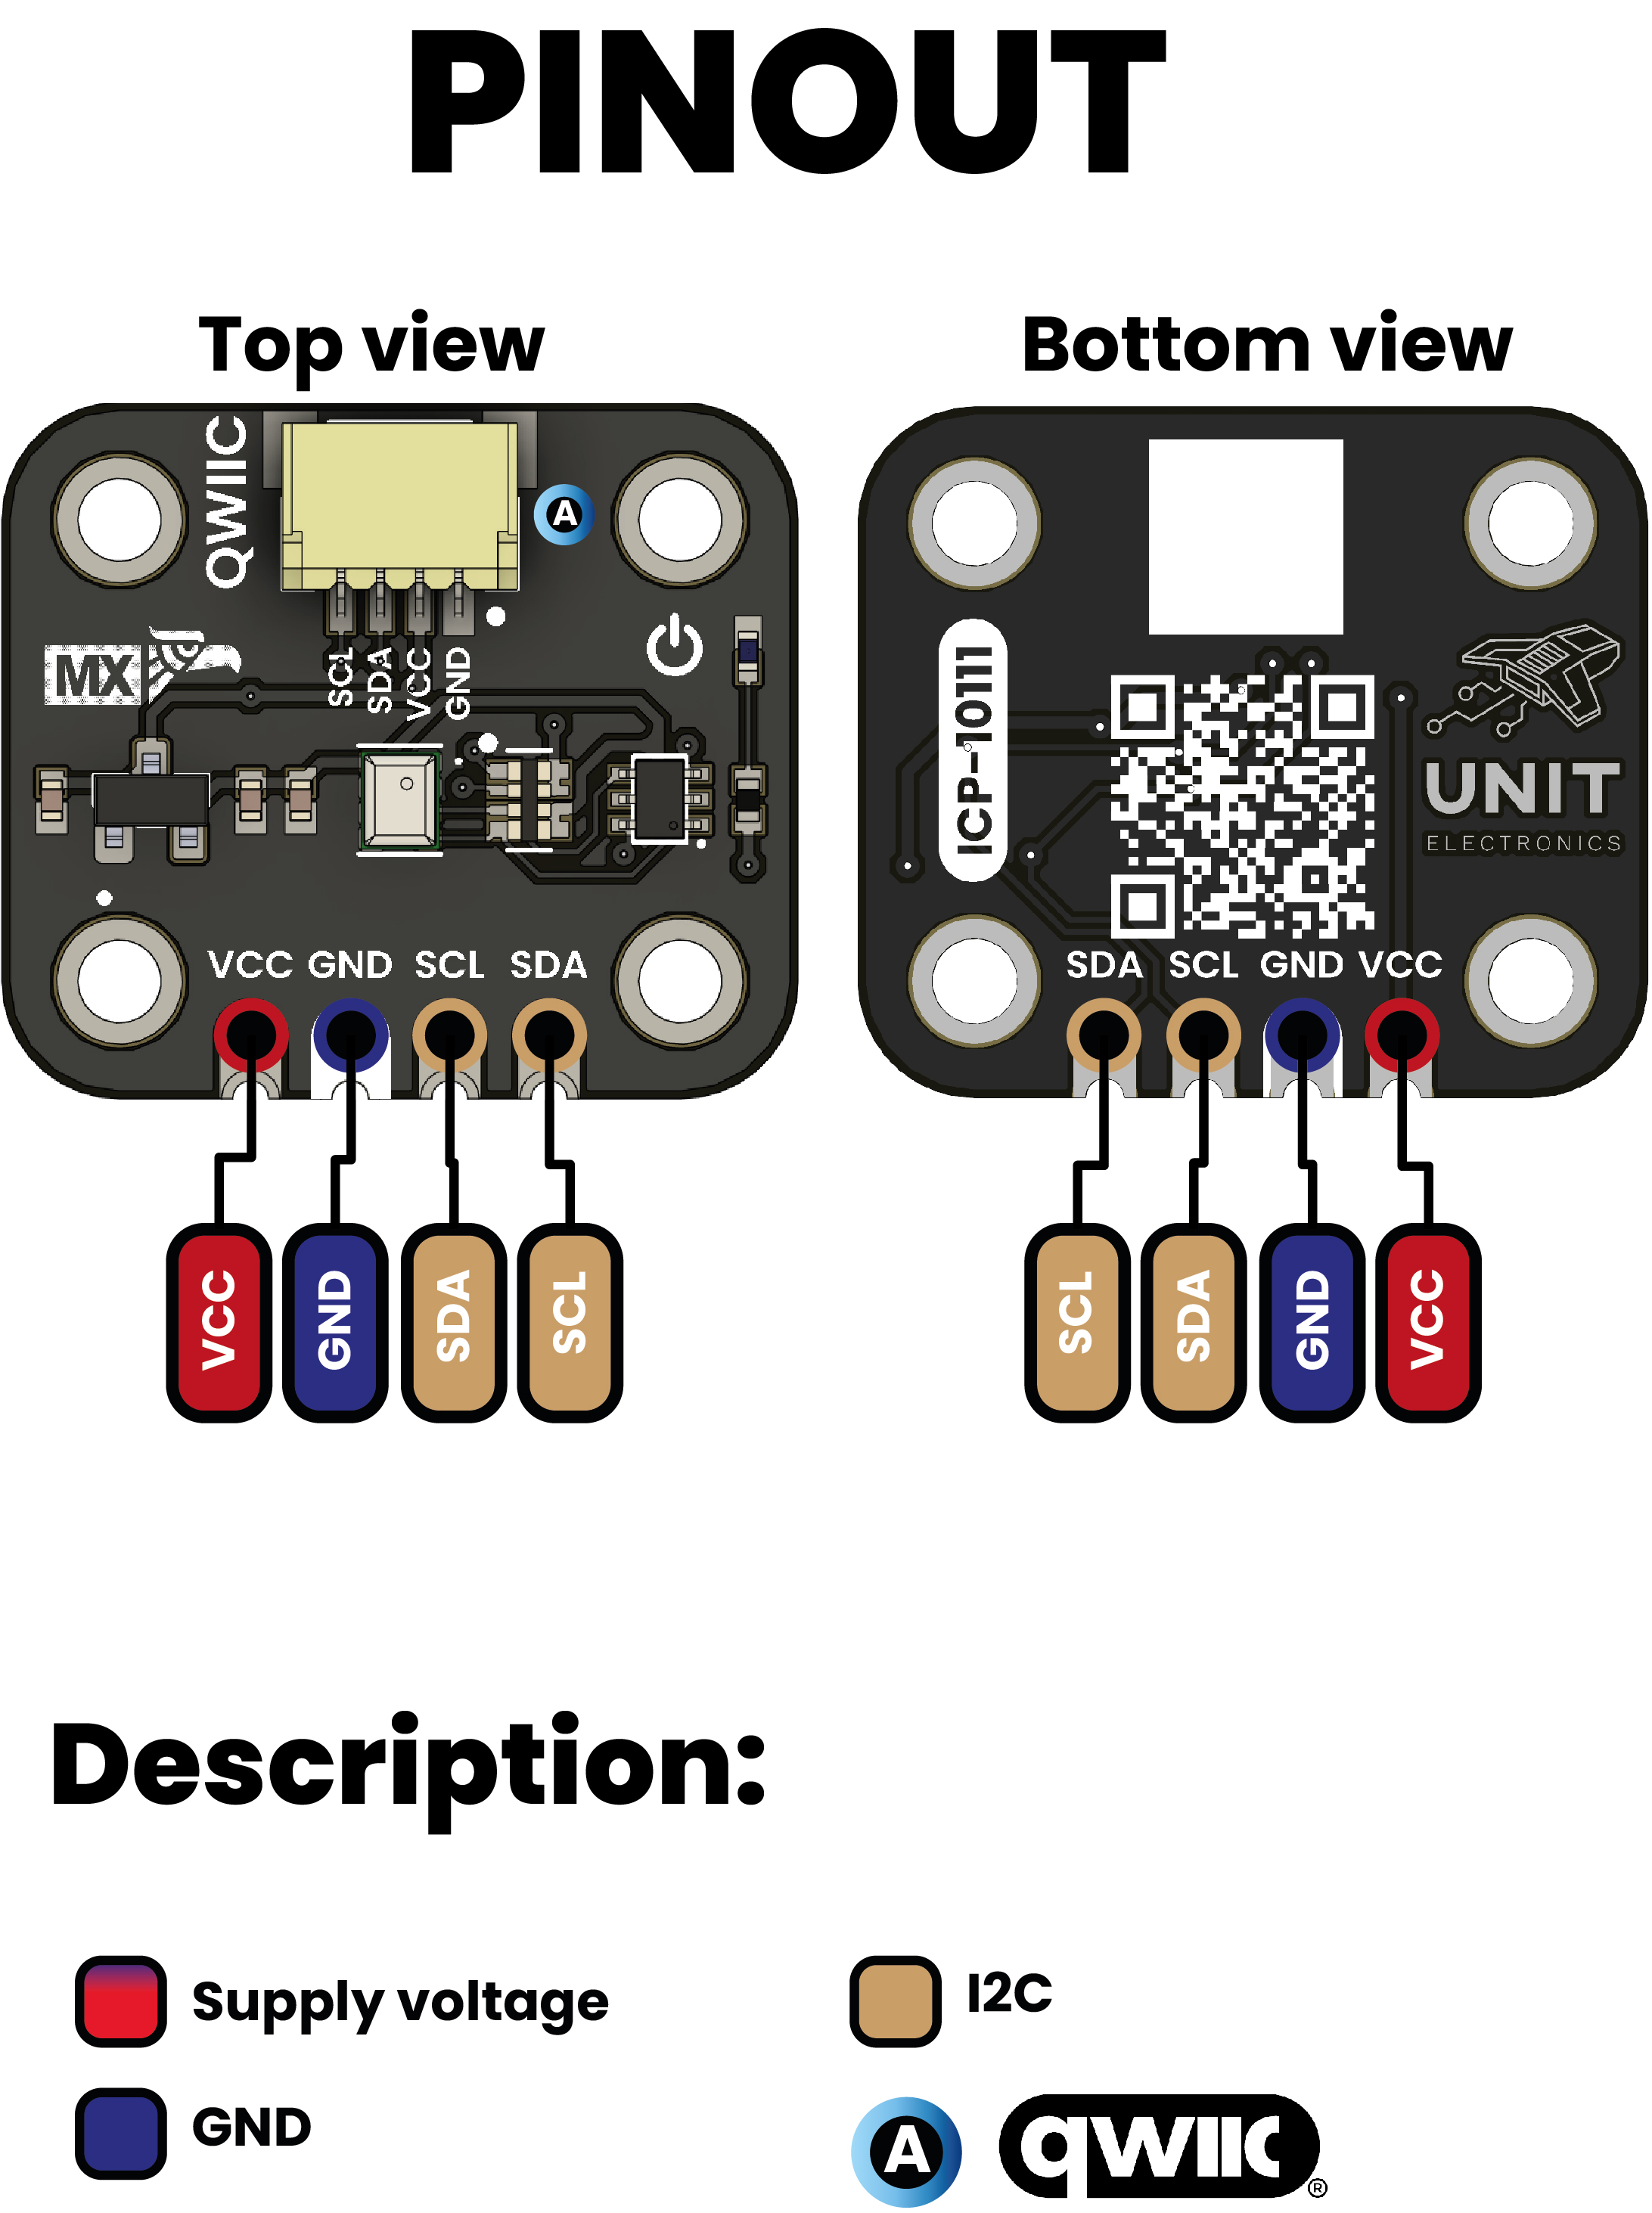
\includegraphics[width=0.9\textwidth]{en_unit_pinout_v_0_0_1_ue0094_icp10111_barometric_pressure_sensor_en.jpg}
\caption{Pinout Diagram}
\label{fig:en-unit-pinout-v-0-0-1-ue0094-icp10111-barometric-pressure-sensor-en-jpg}
\end{figure}




\begin{table}[H]
\centering
\small
\begin{tabular}{|c|c|c|}
\hline
Pin Label & Function & Notes \\
\hline
VCC & Power Supply & 3.3V or 5V \\
GND & Ground & Common ground for all components \\
SDA & I2C Data & Serial data line \\
SCL & I2C Clock & Serial clock line \\
\hline
\end{tabular}
\caption{Especificaciones técnicas}
\end{table}


\subsection{Dimensions}


\begin{figure}[H]
\centering
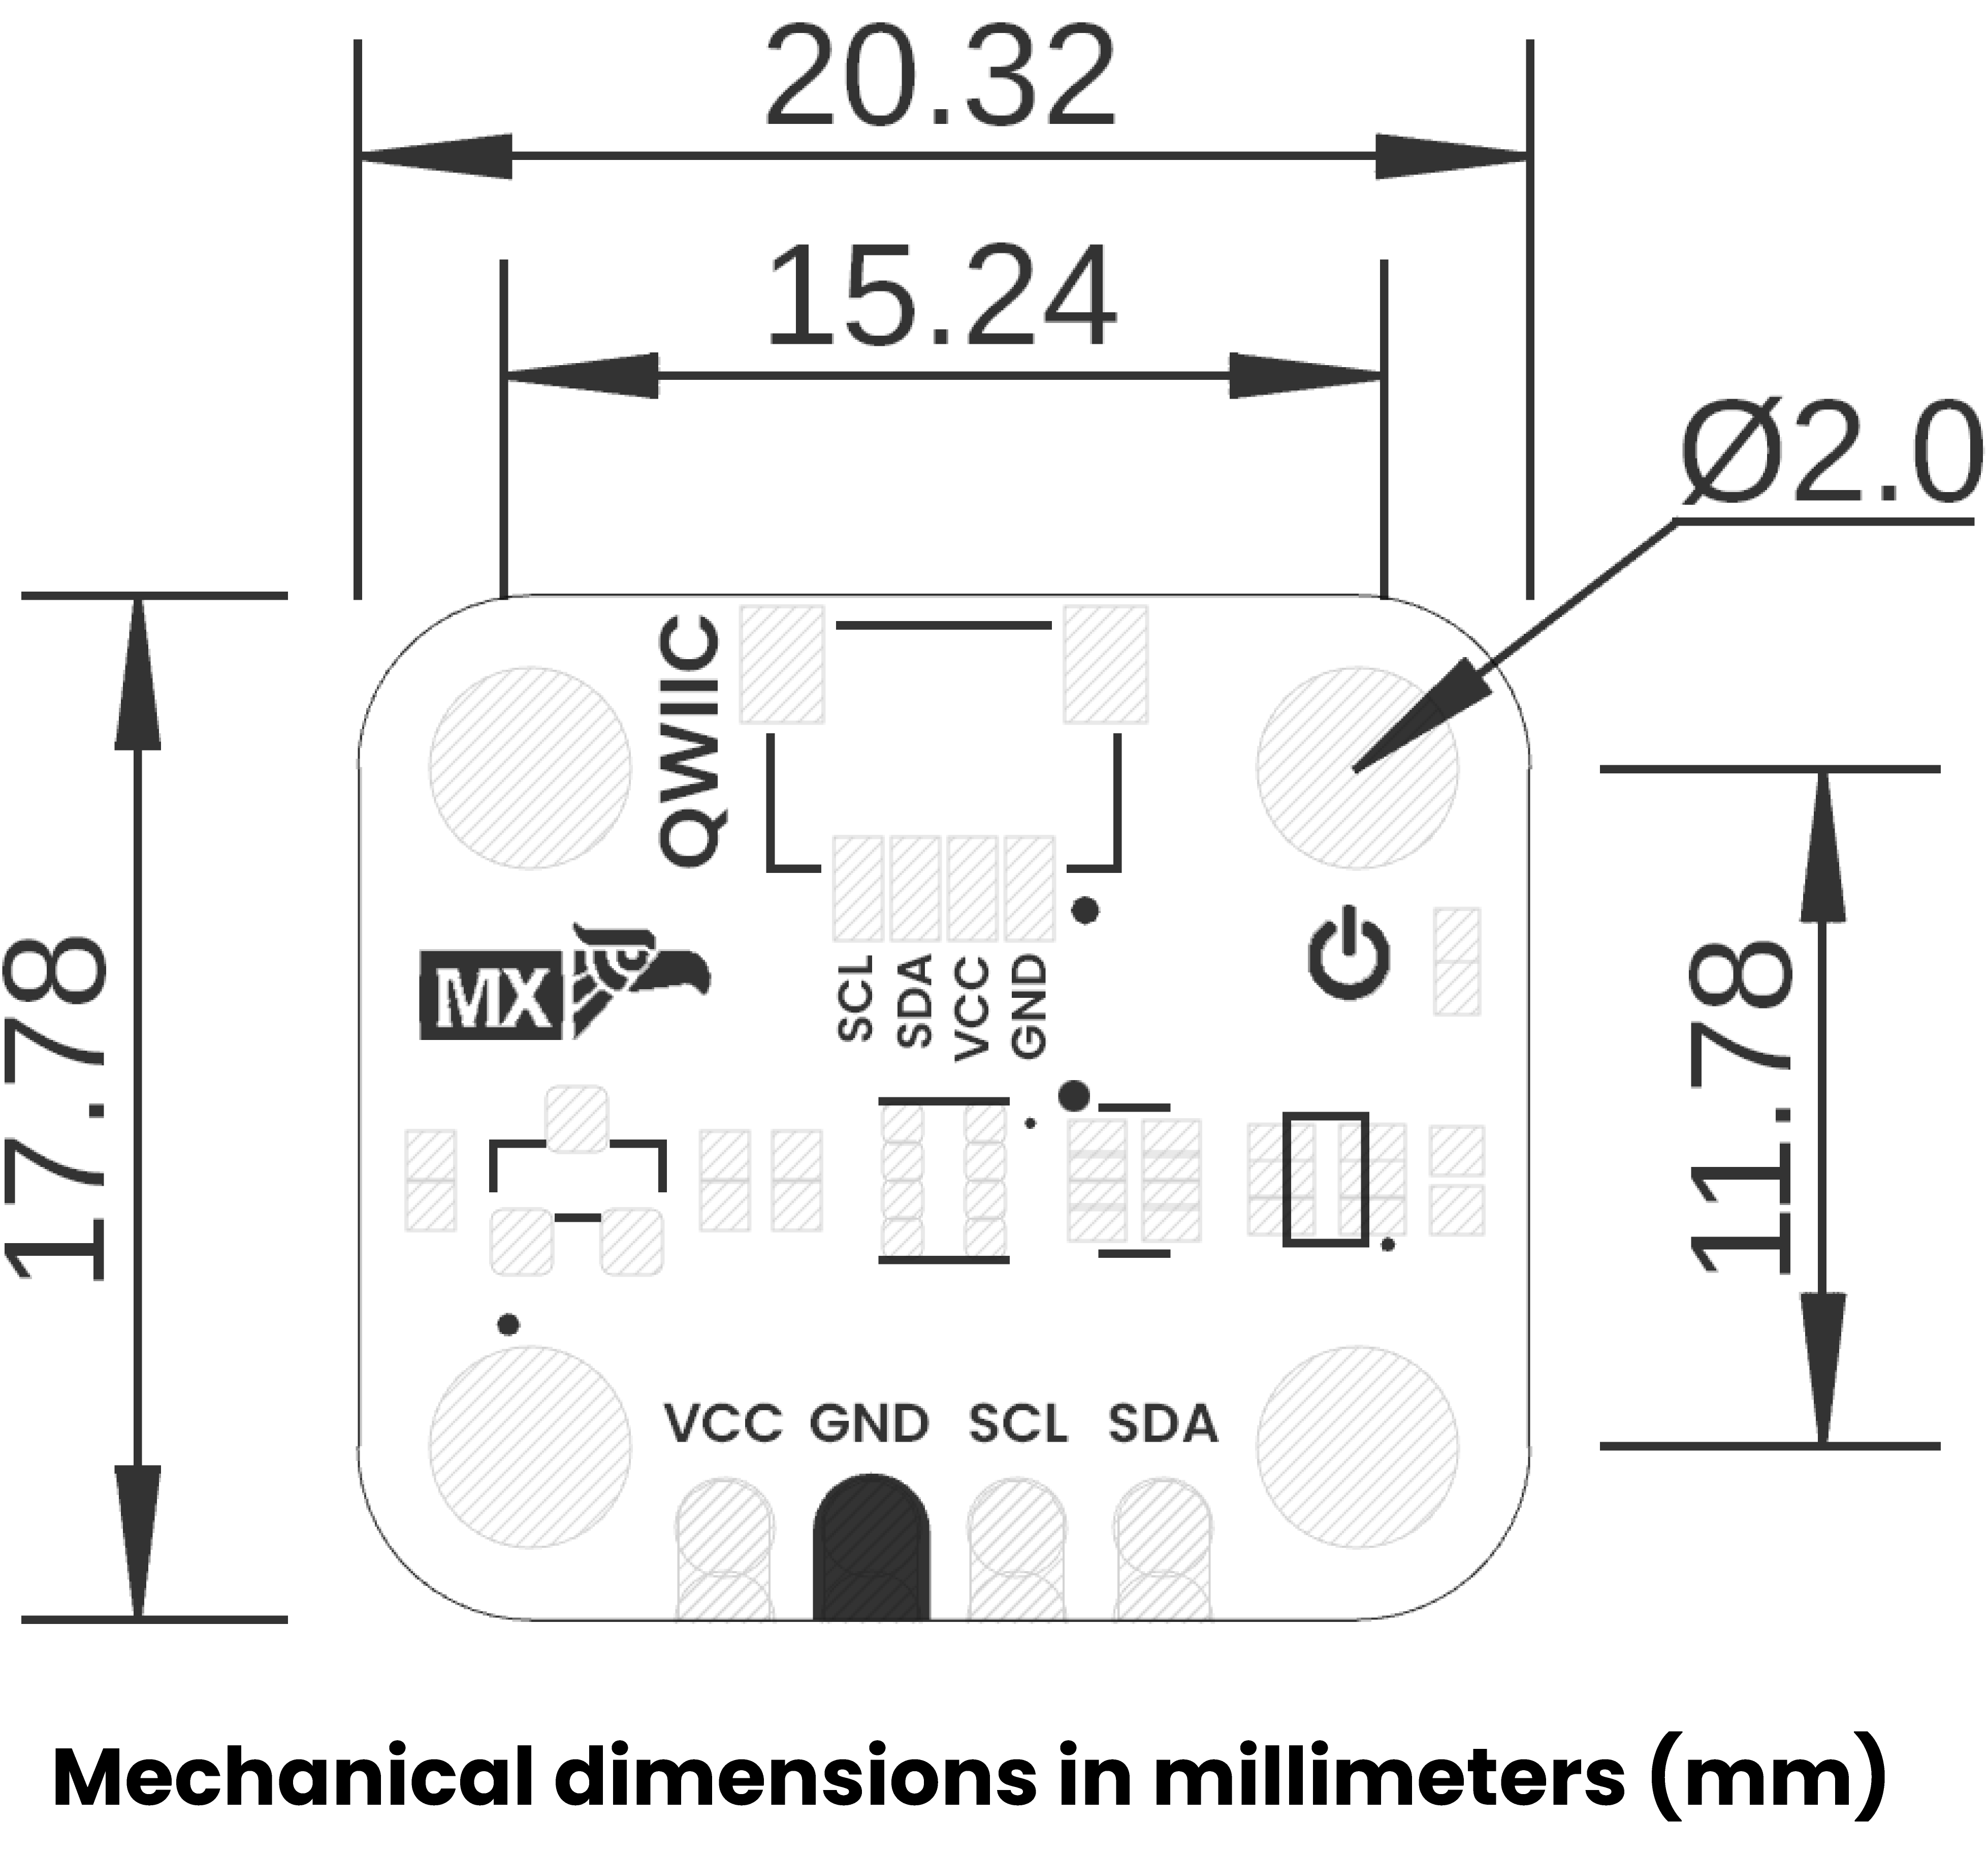
\includegraphics[width=0.6\textwidth]{en_unit_dimension_v_1_0_0_icp10111_barometric_pressure_sensor.png}
\caption{Dimensions}
\label{fig:en-unit-dimension-v-1-0-0-icp10111-barometric-pressure-sensor-png}
\end{figure}



\subsection{Topology}


\begin{figure}[H]
\centering
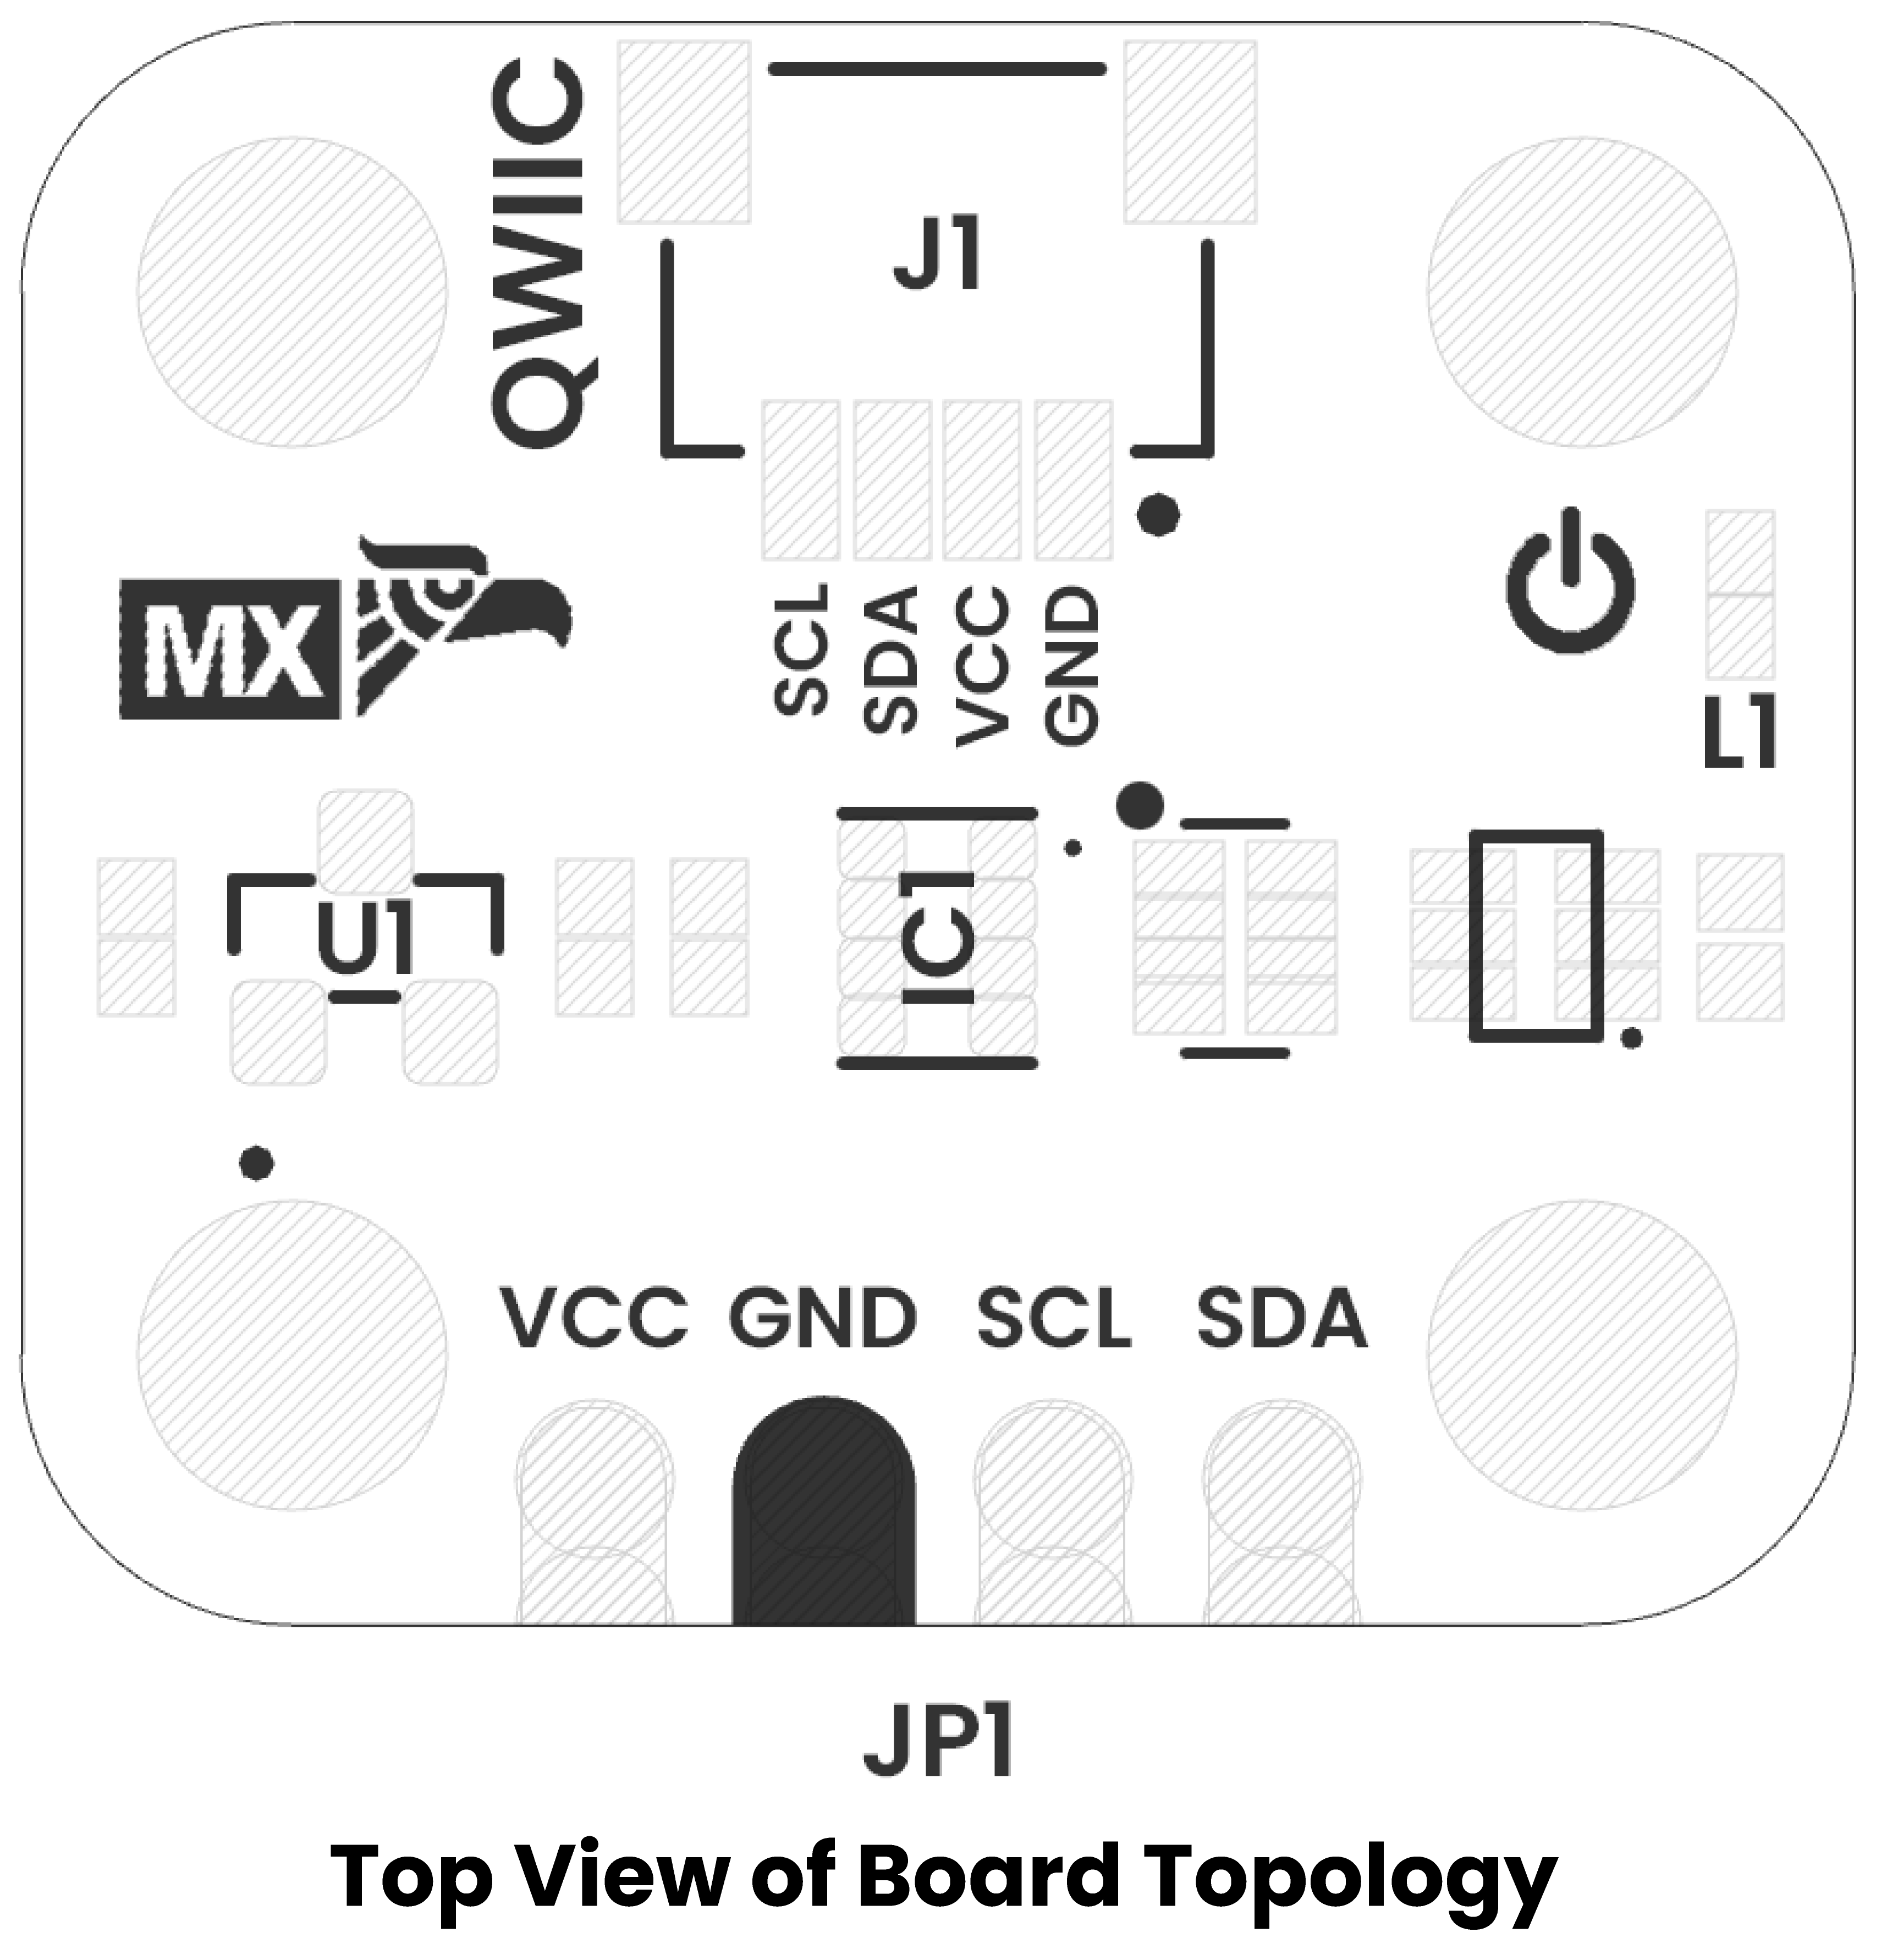
\includegraphics[width=0.7\textwidth]{en_unit_topology_v_1_0_0_icp10111_barometric_pressure_sensor.png}
\caption{Topology}
\label{fig:en-unit-topology-v-1-0-0-icp10111-barometric-pressure-sensor-png}
\end{figure}




\begin{table}[H]
\centering
\small
\begin{tabular}{|c|c|}
\hline
Ref. & Description \\
\hline
IC1 & ICP-10111 Barometric Pressure Sensor \\
IC2 & BME688 Environmental Sensor \\
L1 & Power On LED \\
U1 & ME6206A18XG 1.8V Regulator \\
JP1 & 2.54 mm Castellated Holes \\
J1 & QWIIC Connector (JST 1 mm pitch) for I2C \\
\hline
\end{tabular}
\caption{Especificaciones técnicas}
\end{table}


\subsection{Communication Interfaces}

\subsubsection{I2C Interface}
\begin{itemize}
\item \textbf{Address}: 0x63 (ICP-10111), 0x77 (BME688)
\item \textbf{Speed}: Standard (100 kHz), Fast (400 kHz)
\item \textbf{Features}: QWIIC compatible connector
\item \textbf{Pull-up Resistors}: 4.7k$\Omega$ integrated
\end{itemize}

\subsubsection{Digital Interface Specifications}
\begin{itemize}
\item \textbf{Logic Levels}: 3.3V CMOS compatible
\item \textbf{Input High}: 2.0V minimum
\item \textbf{Input Low}: 0.8V maximum
\item \textbf{Output Drive}: 4mA typical
\end{itemize}

\subsection{Physical Characteristics}

\subsubsection{Package Information}


\begin{table}[H]
\centering
\small
\begin{tabular}{|c|c|c|}
\hline
Parameter & Value & Unit \\
\hline
Package Type & Custom PCB & - \\
Dimensions & 25.4 x 15.24 x 3.2 & mm \\
Mounting & Castellated holes & 2.54mm pitch \\
Weight & 2.1 & g \\
\hline
\end{tabular}
\caption{Especificaciones técnicas}
\end{table}


\subsubsection{Environmental Specifications}


\begin{table}[H]
\centering
\small
\begin{tabular}{|l|l|l|l|l|}
\hline
Parameter & Min & Max & Unit & Conditions \\
\hline
Operating Temperature & -40 & +85 & \degreeC & Full accuracy \\
Storage Temperature & -55 & +125 & \degreeC & - \\
Humidity & 0 & 100 & %RH & Non-condensing \\
Pressure Range & 300 & 1250 & hPa & Absolute pressure \\
\hline
\end{tabular}
\caption{Especificaciones técnicas}
\end{table}


\subsection{Software Support}

\subsubsection{Development Environment}
\begin{itemize}
\item \textbf{Arduino IDE}: Full library support
\item \textbf{ESP-IDF}: Native driver integration
\item \textbf{PlatformIO}: Cross-platform support
\item \textbf{CircuitPython}: Python library available
\end{itemize}

\subsubsection{Key Libraries}
\begin{itemize}
\item ICP-10111 pressure sensor driver
\item BME688 environmental sensor library
\item I2C communication protocols
\item Data filtering and calibration
\end{itemize}

\subsection{Applications}

The ICP-10111 module is ideal for:

\begin{enumerate}
\item \textbf{Weather Monitoring}
\end{enumerate}
\begin{itemize}
\item Atmospheric pressure measurement
\item Altitude determination
\item Weather prediction systems
\end{itemize}

\begin{enumerate}
\item \textbf{IoT Environmental Sensing}
\end{enumerate}
\begin{itemize}
\item Smart building automation
\item Agricultural monitoring
\item Air quality assessment
\end{itemize}

\begin{enumerate}
\item \textbf{Portable Devices}
\end{enumerate}
\begin{itemize}
\item Fitness trackers
\item Outdoor navigation devices
\item Drone altitude control
\end{itemize}

\subsection{Safety and Compliance}

\subsubsection{Certifications}
\begin{itemize}
\item \textbf{RoHS}: Compliant with EU directive
\item \textbf{REACH}: Compliant with EU regulation
\item \textbf{CE}: Electromagnetic compatibility
\end{itemize}

\subsubsection{Safety Features}
\begin{itemize}
\item \textbf{ESD Protection}: $\pm$2kV HBM on all pins
\item \textbf{Reverse Polarity Protection}: Integrated
\item \textbf{Thermal Protection}: Operating range monitoring
\end{itemize}

\subsection{References}

\begin{itemize}
\item \href{https://product.tdk.com/system/files/dam/doc/product/sensor/pressure/capacitive-pressure/data_sheet/ds-000177-icp-10111-v1.3.pdf}{ICP-10111 Datasheet}
\item \href{https://www.bosch-sensortec.com/media/boschsensortec/downloads/datasheets/bst-bme688-ds000.pdf}{BME688 Datasheet}
\item \href{https://www.microne.com.cn/uploads/file/20200904/ME6206.pdf}{ME6206 Regulator Datasheet}
\end{itemize}

\subsection{Ordering Information}


\begin{table}[H]
\centering
\small
\begin{tabular}{|l|l|l|l|}
\hline
Part Number & Description & Package & MOQ \\
\hline
ICP10111-001 & Standard Module & Individual & 1 \\
ICP10111-DEV & Development Kit & Kit Box & 1 \\
ICP10111-BULK & Bulk Order & Tray & 100 \\
\hline
\end{tabular}
\caption{Especificaciones técnicas}
\end{table}


\subsection{Revision History}


\begin{table}[H]
\centering
\small
\begin{tabular}{|c|c|c|}
\hline
Version & Date & Changes \\
\hline
1.0 & 2025-07-18 & Initial release \\
\hline
\end{tabular}
\caption{Especificaciones técnicas}
\end{table}


\subsection{Schematics}


\begin{figure}[H]
\centering

\includegraphics[width=\textwidth]{en_Schematics_icon.jpg}
\caption{Circuit Schematic}
\label{fig:en-Schematics-icon-jpg}
\end{figure}



---

\textit{For technical support and additional information, visit our website or contact our engineering team.}


\end{document}
